% Options for packages loaded elsewhere
\PassOptionsToPackage{unicode}{hyperref}
\PassOptionsToPackage{hyphens}{url}
%
\documentclass[
  ignorenonframetext,
]{beamer}
\usepackage{pgfpages}
\setbeamertemplate{caption}[numbered]
\setbeamertemplate{caption label separator}{: }
\setbeamercolor{caption name}{fg=normal text.fg}
\beamertemplatenavigationsymbolsempty
% Prevent slide breaks in the middle of a paragraph
\widowpenalties 1 10000
\raggedbottom
\setbeamertemplate{part page}{
  \centering
  \begin{beamercolorbox}[sep=16pt,center]{part title}
    \usebeamerfont{part title}\insertpart\par
  \end{beamercolorbox}
}
\setbeamertemplate{section page}{
  \centering
  \begin{beamercolorbox}[sep=12pt,center]{part title}
    \usebeamerfont{section title}\insertsection\par
  \end{beamercolorbox}
}
\setbeamertemplate{subsection page}{
  \centering
  \begin{beamercolorbox}[sep=8pt,center]{part title}
    \usebeamerfont{subsection title}\insertsubsection\par
  \end{beamercolorbox}
}
\AtBeginPart{
  \frame{\partpage}
}
\AtBeginSection{
  \ifbibliography
  \else
    \frame{\sectionpage}
  \fi
}
\AtBeginSubsection{
  \frame{\subsectionpage}
}

\usepackage{amsmath,amssymb}
\usepackage{iftex}
\ifPDFTeX
  \usepackage[T1]{fontenc}
  \usepackage[utf8]{inputenc}
  \usepackage{textcomp} % provide euro and other symbols
\else % if luatex or xetex
  \usepackage{unicode-math}
  \defaultfontfeatures{Scale=MatchLowercase}
  \defaultfontfeatures[\rmfamily]{Ligatures=TeX,Scale=1}
\fi
\usepackage{lmodern}
\usetheme[]{metropolis}
\ifPDFTeX\else  
    % xetex/luatex font selection
\fi
% Use upquote if available, for straight quotes in verbatim environments
\IfFileExists{upquote.sty}{\usepackage{upquote}}{}
\IfFileExists{microtype.sty}{% use microtype if available
  \usepackage[]{microtype}
  \UseMicrotypeSet[protrusion]{basicmath} % disable protrusion for tt fonts
}{}
\makeatletter
\@ifundefined{KOMAClassName}{% if non-KOMA class
  \IfFileExists{parskip.sty}{%
    \usepackage{parskip}
  }{% else
    \setlength{\parindent}{0pt}
    \setlength{\parskip}{6pt plus 2pt minus 1pt}}
}{% if KOMA class
  \KOMAoptions{parskip=half}}
\makeatother
\usepackage{xcolor}
\newif\ifbibliography
\setlength{\emergencystretch}{3em} % prevent overfull lines
\setcounter{secnumdepth}{-\maxdimen} % remove section numbering


\providecommand{\tightlist}{%
  \setlength{\itemsep}{0pt}\setlength{\parskip}{0pt}}\usepackage{longtable,booktabs,array}
\usepackage{calc} % for calculating minipage widths
\usepackage{caption}
% Make caption package work with longtable
\makeatletter
\def\fnum@table{\tablename~\thetable}
\makeatother
\usepackage{graphicx}
\makeatletter
\def\maxwidth{\ifdim\Gin@nat@width>\linewidth\linewidth\else\Gin@nat@width\fi}
\def\maxheight{\ifdim\Gin@nat@height>\textheight\textheight\else\Gin@nat@height\fi}
\makeatother
% Scale images if necessary, so that they will not overflow the page
% margins by default, and it is still possible to overwrite the defaults
% using explicit options in \includegraphics[width, height, ...]{}
\setkeys{Gin}{width=\maxwidth,height=\maxheight,keepaspectratio}
% Set default figure placement to htbp
\makeatletter
\def\fps@figure{htbp}
\makeatother

\makeatletter
\@ifpackageloaded{caption}{}{\usepackage{caption}}
\AtBeginDocument{%
\ifdefined\contentsname
  \renewcommand*\contentsname{Table of contents}
\else
  \newcommand\contentsname{Table of contents}
\fi
\ifdefined\listfigurename
  \renewcommand*\listfigurename{List of Figures}
\else
  \newcommand\listfigurename{List of Figures}
\fi
\ifdefined\listtablename
  \renewcommand*\listtablename{List of Tables}
\else
  \newcommand\listtablename{List of Tables}
\fi
\ifdefined\figurename
  \renewcommand*\figurename{Figure}
\else
  \newcommand\figurename{Figure}
\fi
\ifdefined\tablename
  \renewcommand*\tablename{Table}
\else
  \newcommand\tablename{Table}
\fi
}
\@ifpackageloaded{float}{}{\usepackage{float}}
\floatstyle{ruled}
\@ifundefined{c@chapter}{\newfloat{codelisting}{h}{lop}}{\newfloat{codelisting}{h}{lop}[chapter]}
\floatname{codelisting}{Listing}
\newcommand*\listoflistings{\listof{codelisting}{List of Listings}}
\makeatother
\makeatletter
\makeatother
\makeatletter
\@ifpackageloaded{caption}{}{\usepackage{caption}}
\@ifpackageloaded{subcaption}{}{\usepackage{subcaption}}
\makeatother

\ifLuaTeX
  \usepackage{selnolig}  % disable illegal ligatures
\fi
\usepackage{bookmark}

\IfFileExists{xurl.sty}{\usepackage{xurl}}{} % add URL line breaks if available
\urlstyle{same} % disable monospaced font for URLs
\hypersetup{
  pdftitle={Untitled},
  hidelinks,
  pdfcreator={LaTeX via pandoc}}


\title{Untitled}
\author{}
\date{}

\begin{document}
\frame{\titlepage}


\begin{frame}
\begin{columns}[T]
\begin{column}{0.5\textwidth}
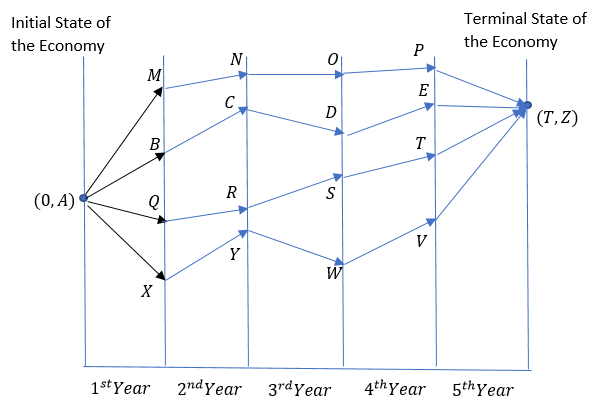
\includegraphics[width=4\textwidth,height=\textheight]{images/do_paths.png}
\end{column}

\begin{column}{0.5\textwidth}
\begin{itemize}
\tightlist
\item
  Suppose the economy starts at \((0,A)\) and wants to reach \((T,Z)\),
  the decision variable will be \textbf{investment in each period}.
\item
  There are different paths to reach the terminal state from the initial
  state.
\end{itemize}
\end{column}
\end{columns}
\end{frame}

\begin{frame}{}
\phantomsection\label{section}
\begin{columns}[T]
\begin{column}{0.7\textwidth}
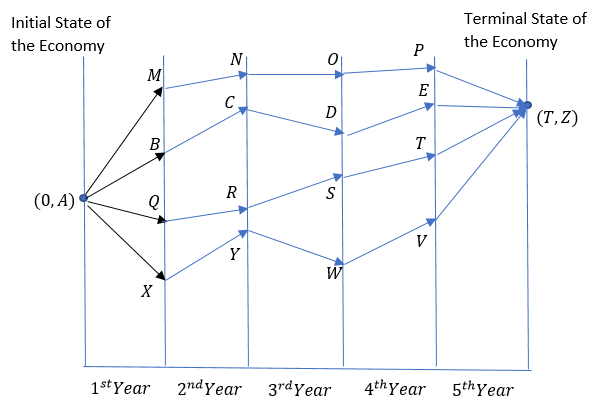
\includegraphics[width=4\textwidth,height=\textheight]{images/do_paths.png}
\end{column}

\begin{column}{0.3\textwidth}
\begin{itemize}
\tightlist
\item
  The question is- which path to select?
\item
  The initial thought might be to choose the path \(A \to X\).
\item
  However, the total cost along the entire path must be considered while
  choosing the optimal path.
\end{itemize}
\end{column}
\end{columns}
\end{frame}

\begin{frame}{}
\phantomsection\label{section-1}
\begin{columns}[T]
\begin{column}{0.7\textwidth}
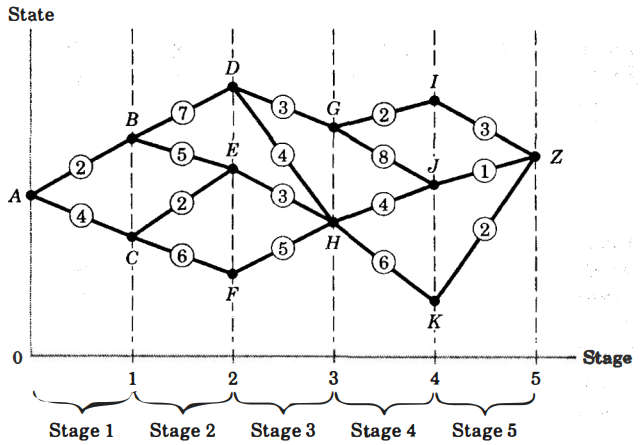
\includegraphics[width=4\textwidth,height=\textheight]{images/do_paths_complex.png}
\end{column}

\begin{column}{0.3\textwidth}
\begin{itemize}
\tightlist
\item
  Consider a more complex path structure.
\item
  Here costs (in billions of ₹) are represented in circles.
\item
  In this case, the path \(ACEHJZ\) gives the optimal solution with
  \(₹14\) billion as the minimum cost.
\end{itemize}
\end{column}
\end{columns}
\end{frame}

\begin{frame}{}
\phantomsection\label{section-2}
\begin{columns}[T]
\begin{column}{0.7\textwidth}
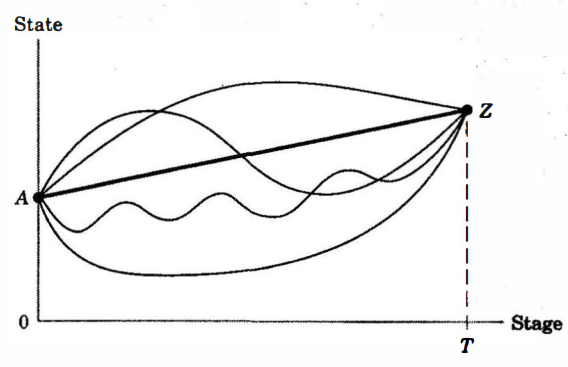
\includegraphics[width=4\textwidth,height=\textheight]{images/do_paths_continuous.png}
\end{column}

\begin{column}{0.3\textwidth}
\begin{itemize}
\tightlist
\item
  This is the continuous variable version.
\item
  Each possible path is seen to travel through an infinite number of
  stages in the interval \([0, T]\).
\item
  E.g. to transport a load of cargo from location \(A\) to \(Z\) at
  minimum travel cost by selecting an appropriate travel path.
\end{itemize}
\end{column}
\end{columns}
\end{frame}

\begin{frame}{Important elements of DO}
\phantomsection\label{important-elements-of-do}
\begin{enumerate}
\tightlist
\item
  In DO, we have initial state \([0,A]\) and terminal state \([T, Z]\).
\item
  There are different paths to achieve the terminal state.
\item
  There should be a \textbf{decision variable}. In our example, it's
  investment.
\item
  We should have an \textbf{objective functional} which we are trying to
  optimize.
\end{enumerate}
\end{frame}

\begin{frame}{Objective function vs objective functional}
\phantomsection\label{objective-function-vs-objective-functional}
\begin{columns}[T]
\begin{column}{0.6\textwidth}
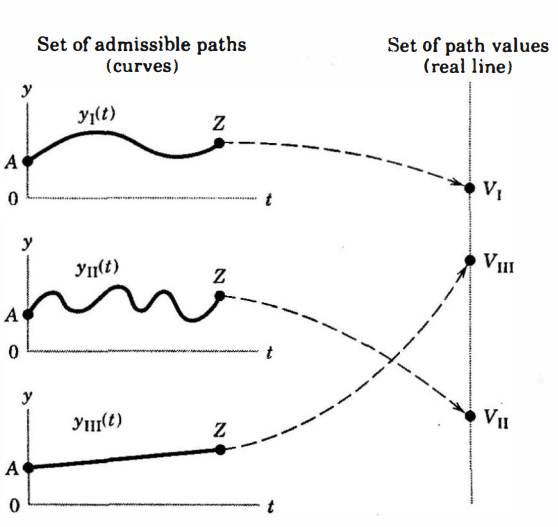
\includegraphics[width=2\textwidth,height=\textheight]{images/do_functional.png}
\end{column}

\begin{column}{0.4\textwidth}
\begin{itemize}
\item
  A function maps elements from one set (the domain) to another set (the
  codomain). For example, \(f(x) = x²\) maps real numbers to real
  numbers.
\item
  A functional, on the other hand, is a special type of function that
  takes another function as its input and returns a number (or more
  generally, a scalar value) as its output. In other words, a functional
  is a \textbf{``function of functions.''}
\end{itemize}
\end{column}
\end{columns}
\end{frame}

\begin{frame}{}
\phantomsection\label{section-3}
\begin{itemize}
\tightlist
\item
  Examples:-

  \begin{enumerate}
  \tightlist
  \item
    The definite integral is a functional:
  \end{enumerate}

  \begin{itemize}
  \tightlist
  \item
    Input: A function \(f(x)\)
  \item
    Output: A single number representing the area under \(f(x)\)
  \item
    Example: \(∫₀¹ f(x)dx\) takes any function f and returns its
    integral from 0 to 1
  \end{itemize}

  \begin{enumerate}
  \setcounter{enumi}{1}
  \tightlist
  \item
    The maximum value functional:
  \end{enumerate}

  \begin{itemize}
  \tightlist
  \item
    Input: A function \(f(x)\) defined on an interval \([a,b]\)
  \item
    Output: The maximum value of \(f(x)\) on that interval
  \item
    Example: \(max{f(x): x ∈ [0,1]}\) takes a function and returns its
    highest value
  \end{itemize}

  \begin{enumerate}
  \setcounter{enumi}{2}
  \tightlist
  \item
    The norm of a function is a functional:
  \end{enumerate}

  \begin{itemize}
  \tightlist
  \item
    Input: A function \(f(x)\)
  \item
    Output: A non-negative real number measuring the ``size'' of the
    function
  \item
    Example: \(L₂ norm: ||f|| = √(∫|f(x)|²dx)\)
  \end{itemize}
\end{itemize}
\end{frame}

\begin{frame}
\begin{itemize}
\item
  Functionals are particularly important when finding the shortest path
  between two points on a surface, we're actually minimizing a
  functional that takes a path (which is a function) as input and
  returns its length as output.
\item
  A key distinction is that functions operate on points (numbers,
  vectors, etc.), while functionals operate on entire functions. This
  makes functionals particularly useful in:

  \begin{itemize}
  \tightlist
  \item
    Optimization problems where we're looking for optimal functions
    rather than optimal points
  \end{itemize}
\end{itemize}
\end{frame}

\begin{frame}{}
\phantomsection\label{section-4}
\begin{columns}[T]
\begin{column}{0.6\textwidth}
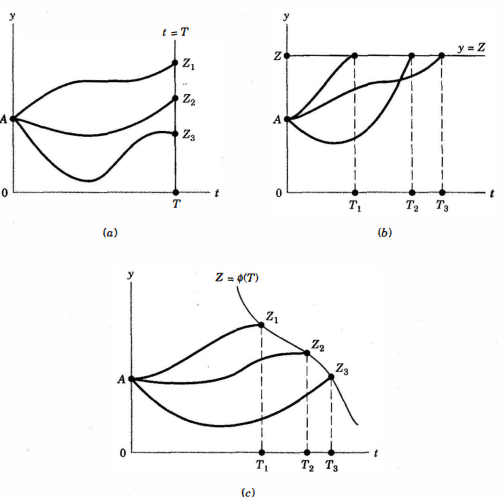
\includegraphics[width=2\textwidth,height=\textheight]{images/do_variable.png}
\end{column}

\begin{column}{0.4\textwidth}
\begin{itemize}
\tightlist
\item
  We might apparently feel that \([0, A]\) and \([T, Z]\) are fixed. But
  this is not the case.
\item
  Either \(T\) or \(Z\) or both may be variable in DO.
\item
  There are alternatives regarding the \textbf{terminal situation}.
\end{itemize}
\end{column}
\end{columns}
\end{frame}

\begin{frame}{Dynamic Optimization}
\phantomsection\label{dynamic-optimization}
\begin{itemize}
\item
  Let us assume we have an asset/resource stock from which we want to
  derive 2 types of benefits:

  \begin{enumerate}
  \tightlist
  \item
    \textbf{Flow benefit}: the value assumed during the use period of
    the resource.
  \item
    \textbf{Scrap value}: the value derived from a resource after it
    becomes obsolete. E.g.a car sold after 20 years or more as scrap.
  \end{enumerate}
\item
  Our objective is to maximize the \textbf{total benefit (flow + scrap
  value)} from the resource.
\item
  Let us denote

  \(V\) : flow benefit

  \(F\) : the scrap value
\end{itemize}
\end{frame}

\begin{frame}
\(\therefore\) Our objective is to

\begin{equation}
\text{max}_{[y(t)]} \ \int_0^T[V(y(t), X(t), t)]dt + F(X(T)) \\
\end{equation}

\begin{align}
\text{s.t.}\ \frac{d X(t)}{d t} = \dot{X}(t) &= f(y(t), X(t)) \ \to \text{equation of motion}\\
& \qquad \qquad \qquad \qquad \text{or dynamic constraint}\\
X(0) &= a \ \to \text{constant}
\end{align}

where;

\begin{align}
F(X(T)) &: \text{scrap value which is realised at the end of the time i.e. T.}\\
y(t) &: \text{decision variable or control variable (e.g. rate of extraction)}\\
X(t) &: \text{state variable i.e. stock of resource at time t.}\\
T &:\text{point of time when scrap value is realised.}\\
t &: \text{continuous time}
\end{align}
\end{frame}

\begin{frame}
To maximise the objective functional we will set a Lagrangian function:

\begin{align}
L &= \int_0^T[V(\cdot) + \lambda(t)\{f(\cdot) - \dot{X}(t)\}]dt + F(X(T))\\
  &= \int_0^T[V(\cdot) + \lambda(t)f(\cdot) - \lambda(t)\dot{X}(t)]dt + F(X(T)) \ \dots (1)
\end{align}

\begin{columns}[T]
\begin{column}{0.4\textwidth}
Consider;

\begin{align}
-\int_0^T \lambda(t)\ \dot{X}(t)dt
\end{align}

The standard integration by parts formula is:

\begin{equation}
\int u \frac{dv}{dt} dt = u \cdot v - \int v \frac{du}{dt} dt
\end{equation}
\end{column}

\begin{column}{0.55\textwidth}
Let \(u = \lambda(t)\)

Let \(dv = \dot{X}(t)dt\)

\(\frac{du}{dt} = \dot{\lambda}(t)\)

\(v = X(t)\)

\begin{align}
-\int_0^T \lambda(t)\ \dot{X}(t)dt &= -[\lambda(t)X(t)]_0^T + \int_0^T X(t)\dot{\lambda}(t)dt \\
&= -\lambda(T)X(T) + \lambda(0)X(0) + \int_0^T X(t)\dot{\lambda}(t)dt\\
\end{align}
\end{column}
\end{columns}
\end{frame}

\begin{frame}
\begin{align}
\therefore -\int_0^T \lambda(t)\ \dot{X}(t)dt &= -[\lambda(t)X(t)]_0^T + \int_0^T X(t)\dot{\lambda}(t)dt \\
&= -\lambda(T)X(T) + \lambda(0)X(0) + \int_0^T X(t)\dot{\lambda}(t)dt \ \dots (2)
\end{align}

Recall;

\begin{align}
L &= \int_0^T[V(\cdot) + \lambda(t)f(\cdot) - \lambda(t)\dot{X}(t)]dt + F(X(T))\ \dots (1)
\end{align}

Substituting the result from equation (2):

\begin{align}
L &= \int_0^T[V(\cdot) + \lambda(t)f(\cdot)]dt - \lambda(T)X(T) + \lambda(0)X(0) + \int_0^T X(t)\dot{\lambda}(t)dt + F(X(T)) \ \dots (3)
\end{align}
\end{frame}

\begin{frame}
Let us define

\begin{align}
H &= V(\cdot) + \lambda(t)f(\cdot) \\
\implies H &= H(y(t), X(t), \lambda(t), t)
\end{align}

\begin{align}
\therefore L &= \int_0^T[H(\cdot)]dt - \lambda(T)X(T) + \lambda(0)X(0) + \int_0^T X(t)\dot{\lambda}(t)dt + F(X(T)) \\
&= \int_0^T[H(\cdot)]dt  + \int_0^T X(t)\dot{\lambda}(t)dt + F(X(T)- \lambda(T)X(T) + \lambda(0)X(0)) \\
&= \int_0^T\left[H(\cdot)  + X(t)\dot{\lambda}(t)\right]dt + F(X(T)- \lambda(T)X(T) + \lambda(0)X(0))
\end{align}

We want to optimize \(L\) by chosing \(y(t)\) the control variable.

Let us assume \(y(t)\) is changed to \(y(t) + \Delta y(t)\)

\(\{y(t) \to y(t) + \Delta y(t)\}\): \textbf{Change in the rate of
extraction.}

\(\{X(t) \to X(t) + \Delta X(t)\}\): \textbf{Change in the stock of
resources.}
\end{frame}

\begin{frame}{Step 1: Define \(L\)}
\phantomsection\label{step-1-define-l}
The given functional is:

\[
L = \int_0^T\left[H(\cdot)  + X(t)\dot{\lambda}(t)\right]dt + F(X(T)- \lambda(T)X(T) + \lambda(0)X(0))
\]

where:

\begin{itemize}
\tightlist
\item
  \(H(\cdot)\) is the \textbf{Hamiltonian}.
\item
  \(X(t)\) is the \textbf{state variable}.
\item
  \(\lambda(t)\) is the \textbf{co-state (Lagrange multiplier)}.
\item
  \(F(\cdot)\) is a function depending on the terminal state \(X(T)\).
\end{itemize}
\end{frame}

\begin{frame}{Why is it called the Hamiltonian?}
\phantomsection\label{why-is-it-called-the-hamiltonian}
The \textbf{Hamiltonian} is named after \textbf{Sir William Rowan
Hamilton}, who developed \textbf{Hamiltonian mechanics} in the 19th
century. Originally, it was used in \textbf{classical mechanics} to
describe the total energy of a system:

In Physics

\begin{align}
H &= T(q, p, t) + V(q, t) \\
\implies \text{Total Energy} &= \text{Kinetic Energy} + \text{Potential Energy}
\end{align}

And in Economics

\begin{align}
H &= V(y(t), X(t), t) + \lambda(t)f(y(t), X(t)) \\ 
\implies \text{Total Benefits or Costs} &= \text{Flow Benefit or Costs} + \text{Stock Benefit or Costs}
\end{align}
\end{frame}

\begin{frame}{Step 2: Compute the Variation \(\Delta L\)}
\phantomsection\label{step-2-compute-the-variation-delta-l}
The total variation of \(L\) comes from two parts:

\begin{enumerate}
\tightlist
\item
  \textbf{Variation of the Integral Term}: \[
  \int_0^T \left[H(\cdot) + X(t)\dot{\lambda}(t)\right] dt
  \]
\item
  \textbf{Variation of the Terminal Function \(F(\cdot)\)}: \[
  F(X(T)- \lambda(T)X(T) + \lambda(0)X(0))
  \]
\end{enumerate}
\end{frame}

\begin{frame}{Step 2.1: Variation of the Integral Term}
\phantomsection\label{step-2.1-variation-of-the-integral-term}
Since \(L\) is an integral, its variation follows:

\[
\Delta L = \int_0^T \Delta \left[ H(\cdot) + X(t)\dot{\lambda}(t) \right] dt + \Delta F(\cdot)
\]

Expanding \(\Delta H(\cdot)\) using the \textbf{first-order Taylor
expansion}:

\[
\Delta H(\cdot) = \frac{\partial H}{\partial y(t)} \Delta y(t) + \frac{\partial H}{\partial X(t)} \Delta X(t)
\]

Also, the variation of \(X(t) \dot{\lambda}(t)\) gives:

\[
\Delta (X(t) \dot{\lambda}(t)) = \dot{\lambda}(t) \Delta X(t)
\]

\[
\implies \int_0^T \left[ 
\frac{\partial H}{\partial y(t)} \Delta y(t) + 
\frac{\partial H}{\partial X(t)} \Delta X(t) + 
\dot{\lambda}(t) \Delta X(t)
\right] dt
\]
\end{frame}

\begin{frame}{Step 2.2: Variation of the Terminal Function \(F(\cdot)\)}
\phantomsection\label{step-2.2-variation-of-the-terminal-function-fcdot}
The function \(F(X(T)- \lambda(T)X(T) + \lambda(0)X(0))\) depends on
\(X(T)\), \(\lambda(T)\), and \(X(0)\). Its total variation is:

\[
\Delta F = \frac{\partial F}{\partial X(T)} \Delta X(T) - \lambda(T) \Delta X(T) + \lambda(0) \frac{\partial X(0)}{\partial X(T)} \Delta X(T)
\]

Since \(X(0)\) is \textbf{constant}, its derivative with respect to
\(X(T)\) is:

\[
\frac{\partial X(0)}{\partial X(T)} = 0
\]

which simplifies the terminal term to:

\[
\frac{\partial F}{\partial X(T)} \Delta X(T) - \lambda(T) \Delta X(T)
\]
\end{frame}

\begin{frame}{Step 3: Final Expression for \(\Delta L\)}
\phantomsection\label{step-3-final-expression-for-delta-l}
Now, combining everything:

\[
\Delta L = \int_0^T\left[ 
\frac{\partial H}{\partial y(t)}\Delta y(t) +
\frac{\partial H}{\partial X(t)}\Delta X(t) +
\dot{\lambda}(t) \Delta X(t)
\right]dt
+ \frac{\partial F}{\partial X(T)}\Delta X(T) - \lambda(T)\Delta X(T)
\]
\end{frame}

\begin{frame}
For optimization \textbf{\(\Delta L = 0\)}, we analyze:

\[
\Delta L = \int_0^T\left[ 
\frac{\partial H}{\partial y(t)}\Delta y(t) +
\frac{\partial H}{\partial X(t)}\Delta X(t) +
\dot{\lambda}(t) \Delta X(t)
\right]dt
+ \frac{\partial F}{\partial X(T)}\Delta X(T) - \lambda(T)\Delta X(T)
\]

Rearranging;

\[
\Delta L = \int_0^T\left[ 
\frac{\partial H}{\partial y(t)}\Delta y(t) +
\left(\frac{\partial H}{\partial X(t)} +
\dot{\lambda}(t)\right)\Delta X(t)
\right]dt
+ \left(\frac{\partial F}{\partial X(T)} - \lambda(T)\right)\Delta X(T)
\]

Since \textbf{\(\Delta L = 0\)} must hold for any small variations
\textbf{\(\Delta X(t)\)} and \textbf{\(\Delta y(t)\)}, each coefficient
must be zero.
\end{frame}

\begin{frame}{Principle 1}
\phantomsection\label{principle-1}
Since \(\Delta y(t)\) is arbitrary, we must have:

\[\frac{\partial H}{\partial y(t)} = 0\]

This is the \textbf{control optimality condition}, ensuring that the
Hamiltonian is optimized with respect to the control \(y(t)\).
\end{frame}

\begin{frame}{Principle 2}
\phantomsection\label{principle-2}
From the integral term:

\[
\left[\frac{\partial H}{\partial X(t)} + \dot{\lambda}(t)\right] \Delta X(t)
\]

For arbitrary \(\Delta X(t)\), we get:

\[
\dot{\lambda}(t) = -\frac{\partial H}{\partial X(t)}
\]

This is the \textbf{co-state equation}, governing the evolution of the
costate \(\lambda(t)\).
\end{frame}

\begin{frame}{Principle 3}
\phantomsection\label{principle-3}
From the terminal variation term:

\[
\left[\frac{\partial F}{\partial X(T)} - \lambda(T)\right] \Delta X(T)
\]

For arbitrary \(\Delta X(T)\), we get:

\[
\lambda(T) = \frac{\partial F}{\partial X(T)}
\]

This is setting the final value of the costate.
\end{frame}

\begin{frame}{Summary of Maximum Principle Conditions}
\phantomsection\label{summary-of-maximum-principle-conditions}
To satisfy \(\Delta L = 0\):

\begin{enumerate}
\item
  \textbf{Control Optimality Condition}\\
  \[\frac{\partial H}{\partial y(t)} = 0\]
\item
  \textbf{Co-state Equation}\\
  \[\dot{\lambda}(t) = -\frac{\partial H}{\partial X(t)}\]
\item
  \textbf{Terminal Condition}\\
  \[\lambda(T) = \frac{\partial F}{\partial X(T)}\]
\end{enumerate}

These are the necessary conditions from \textbf{Pontryagin's Maximum
Principle}.
\end{frame}

\begin{frame}{\textbf{Pontryagin's Maximum Principle: Interpretation}}
\phantomsection\label{pontryagins-maximum-principle-interpretation}
\begin{itemize}
\tightlist
\item
  Pontryagin's Maximum Principle is named after the Russian
  mathematician Lev Pontryagin, who formulated this principle in 1956
  along with his students.
\item
  The principle was initially developed to solve optimization problems
  in control theory, specifically for maximizing the terminal speed of a
  rocket.
\end{itemize}
\end{frame}

\begin{frame}
\begin{block}{\textbf{1. Control Optimality Condition}}
\phantomsection\label{control-optimality-condition}
\[\frac{\partial H}{\partial y(t)}=0\]

\begin{block}{\textbf{Interpretation:}}
\phantomsection\label{interpretation}
\begin{itemize}
\tightlist
\item
  Ensures that the \textbf{Hamiltonian is optimized} with respect to the
  control variable \(y(t)\).\\
\item
  Determines the \textbf{optimal control strategy}.\\
\item
  The best action \(y^*(t)\) must satisfy this equation.
\end{itemize}
\end{block}

\begin{block}{\textbf{Example (Renewable Resource Extraction)}}
\phantomsection\label{example-renewable-resource-extraction}
\begin{itemize}
\tightlist
\item
  Managing a \textbf{fishery}:

  \begin{itemize}
  \tightlist
  \item
    \(y(t)\) = harvesting rate\\
  \item
    \(X(t)\) = fish population\\
  \item
    \(\frac{\partial H}{\partial y(t)}=0\) ensures \textbf{profit
    maximization while maintaining sustainability}.
  \end{itemize}
\end{itemize}
\end{block}
\end{block}
\end{frame}

\begin{frame}
\begin{block}{\textbf{2. Co-State (Shadow Price) Equation}}
\phantomsection\label{co-state-shadow-price-equation}
\[\dot{\lambda}(t)=-\frac{\partial H}{\partial X(t)}\]

\begin{block}{\textbf{Interpretation:}}
\phantomsection\label{interpretation-1}
\begin{itemize}
\tightlist
\item
  Describes how the \textbf{shadow price \(\lambda(t)\) evolves over
  time}.\\
\item
  \(\lambda(t)\) represents \textbf{the value of an extra unit of
  \(X(t)\)}.\\
\item
  Shows how resource depletion \textbf{affects future value}.
\end{itemize}
\end{block}

\begin{block}{\textbf{Example (Groundwater Extraction)}}
\phantomsection\label{example-groundwater-extraction}
\begin{itemize}
\tightlist
\item
  \(X(t)\) = amount of water in aquifer\\
\item
  \(y(t)\) = extraction rate\\
\item
  \(\lambda(t)\) = future value of preserving water\\
\item
  If overuse today \textbf{reduces future availability}, then
  \(\lambda(t)\) changes accordingly.
\end{itemize}
\end{block}
\end{block}
\end{frame}

\begin{frame}
\begin{block}{\textbf{3. Transversality (Terminal) Condition}}
\phantomsection\label{transversality-terminal-condition}
\[\lambda(T)=\frac{\partial F}{\partial X(T)}\]

\begin{block}{\textbf{Interpretation:}}
\phantomsection\label{interpretation-2}
\begin{itemize}
\tightlist
\item
  Determines the \textbf{final value of shadow price \(\lambda(T)\)}.\\
\item
  If there's a \textbf{terminal reward or penalty}, it sets the final
  condition.\\
\item
  If no terminal condition exists, often \textbf{\(\lambda(T)=0\)}.
\end{itemize}
\end{block}

\begin{block}{\textbf{Example (Deforestation \& Land Use)}}
\phantomsection\label{example-deforestation-land-use}
\begin{itemize}
\tightlist
\item
  \(X(T)\) = remaining forest at time \(T\)
\item
  \(\frac{\partial F}{\partial X(T)}\) = future value of forest\\
\item
  Ensures that \textbf{future benefits of conservation} are included in
  today's decisions.
\end{itemize}
\end{block}
\end{block}
\end{frame}

\begin{frame}
Recall,

\[
H = V(\cdot) + \lambda (t)f(\cdot)
\]

where;

\(V(\cdot)\): flow benefit

\(\lambda (t)f(\cdot)\): future benefit or value

\(\lambda (t)\): shadow price
\end{frame}

\begin{frame}
\(\therefore H = \text{Present Benefit + Future Benefit}\)

Future benefit is realised at one point in time.

However, present benefits are a stream of benefits.

So if we have to convert \(V(\cdot)\) at present time then we have to
multiply it with \(e^{-rt}\), i.e.~discounting.
\end{frame}

\begin{frame}
\(\because H = V(\cdot) + \lambda (t)f(\cdot)\)

\(H_p = V(\cdot)e^{-rt} + \lambda (t)f(\cdot)\)

where;

\(H_p\): Present Value Hamiltonian because the \textbf{flow benefit} is
converted into stock benefit.
\end{frame}

\begin{frame}
Now we want to convert the sotck (one period) benefit into a stream of
benefits:

\(H_c = V(\cdot) + \lambda (t)e^{rt}f(\cdot)\)

where;

\(H_c\): Current Value Hamiltonian because the \textbf{stock (one
period) benefit} is converted to flow benefits.
\end{frame}

\begin{frame}
Let's assume

\begin{align}
\lambda(t)e^{rt} &= \rho (t)\\
\implies \lambda(t) &= \rho(t) e^{-rt} \\
\implies \dot{\lambda}(t) &= \dot{\rho}(t) e^{-rt} - r\rho(t)e^{-rt}\\
\implies \dot{\lambda}(t)e^{rt} &= \dot{\rho}(t)  - r\rho(t)\\ 
\implies \dot{\rho}(t) &= \dot{\lambda}(t)e^{rt} + r\rho(t)
\end{align}

where,

\(\rho(t)\): current value of the co-state variable \(\lambda(t)\)
\end{frame}

\begin{frame}
Intuition:

The idea behind \(H_p\) and \(H_c\) is that we are representing two
types of benefits that we can actually get from a NRR.

These benefits could be flow or stock; and in the Hamiltonian we have
converted either of the benefits (flow or stock) to arrive at a single
benefit (present value) or stream of benefits (current value).
\end{frame}

\begin{frame}
Maximizing total (flow + stock) benefits requires
\end{frame}




\end{document}
